\documentclass[11pt, a4paper]{article}

\usepackage{listings}
\usepackage{subfigure}
\usepackage{graphicx}
\usepackage{titling}
\usepackage[margin=1.9cm, includefoot]{geometry}
%\usepackage{fullpage}
\newcommand{\subtitle}[1]{
  \posttitle{
    \par\end{center}
    \begin{center}\large#1\end{center}
    \vskip0.5em}
}

\setlength{\droptitle}{-4em}

\begin{document}

\title{Deeva}
\subtitle{Planning Report}
\author{Kritaphat Sonsri-in, Xueqi Chen, Hector Dearman, \\Alina Draganescu, Felix de Souza}

\maketitle

\section{The Task}
Our group was assigned to a project to build a simple but powerful Java debugger to help teach first year computing students Java.

Our supervisor Dr.~Tristan Allwood proposed this project for two main reasons.
Firstly although he would like to avoid teaching Java in a way that made students dependent on a `magic' IDE like Eclipse this becomes difficult without a good external debugger like GDB which is for C\footnote{The various external Java debuggers like JDB all have serious bugs and/or usability problems.}.
Secondly many students initially don't have a clear mental picture of what the computer is doing\footnote{Roughly half are programing in an imperative language for the first time.} so it would be good for students to be able to graphically inspect the stack and heap of a running Java program in a similar way to how they are being taught to visualize the stack and heap in lectures.

To fix these problems he envisioned a Java debugger that was: started from the command line (to avoid IDE magic), intuitive enough to used by people who had not previously used a debugger (but powerful enough to be useful) and which could visually display the state of the stack and the heap to help further the development of a mental model of Java.

\section{How we prepared the Plan}

For this project we have three problems which we haven't had (at least in combination) in past university projects: we're not sure what we're building, we want to make sure we deliver the software on time but don't know how long it will take and
we want to make sure the software we write is correct and useful but have no easy way to define `correct' or `useful' in this domain.

Happily Agile programing has techniques we can use to help to solve these problems\footnote{Indeed the first principle of the Agile manifesto is: ``Our highest priority is to satisfy the customer
through early and continuous delivery of valuable software." ({\tt http://agilemanifesto.org/principles.html})which is directly related to our problems.}.

The first part of building good software is to make sure you understand the problem.
As you can see below we went through a few iterations of the plan and are continuing to meet our project owner every week to make sure we build the right thing.

\subsection{0th group meeting}
Immediately after we got a group assignment we had a very short stand up group meeting where we agreed which of us would arrange a meeting with Tristan, set-up Trello and create a Github repository.  

\subsection{First meeting with Tristan}
During the meeting that we arranged with Tristan, we talked through what we had understood from the specification for the project. We also asked him to go through his expectations in detials so that we could get a full understanding on the project. For example, what core functionalities does the debugger need and how it should be used e.g. how it should be started from the command line. We wrote down our  meeting minutes on Google Docs.

\subsection{First group meeting}
After our first meeting with Tristan, we had our first formal group meeting with the information Tristan had provided us. We decided to use Agile Programming as our development methodology as we go along. During the meeting, we came up with some research topics that were necessary for the project such as: tools/frameworks, comparison of different Java debuggers and etc. Everyone picked one story based on their preference with a set deadline. For example, Krit and Kira were working on the comparison of different debuggers. Hector and Felix were researching on frameworks and tools. Alina was assigned with making estimation poker cards and getting the first year Java exercises as reference material. We used Google docs for editing and gathering information that we had found. 

\begin{figure}[ht]
\centering
\subfigure[Planning Poker Game]{%
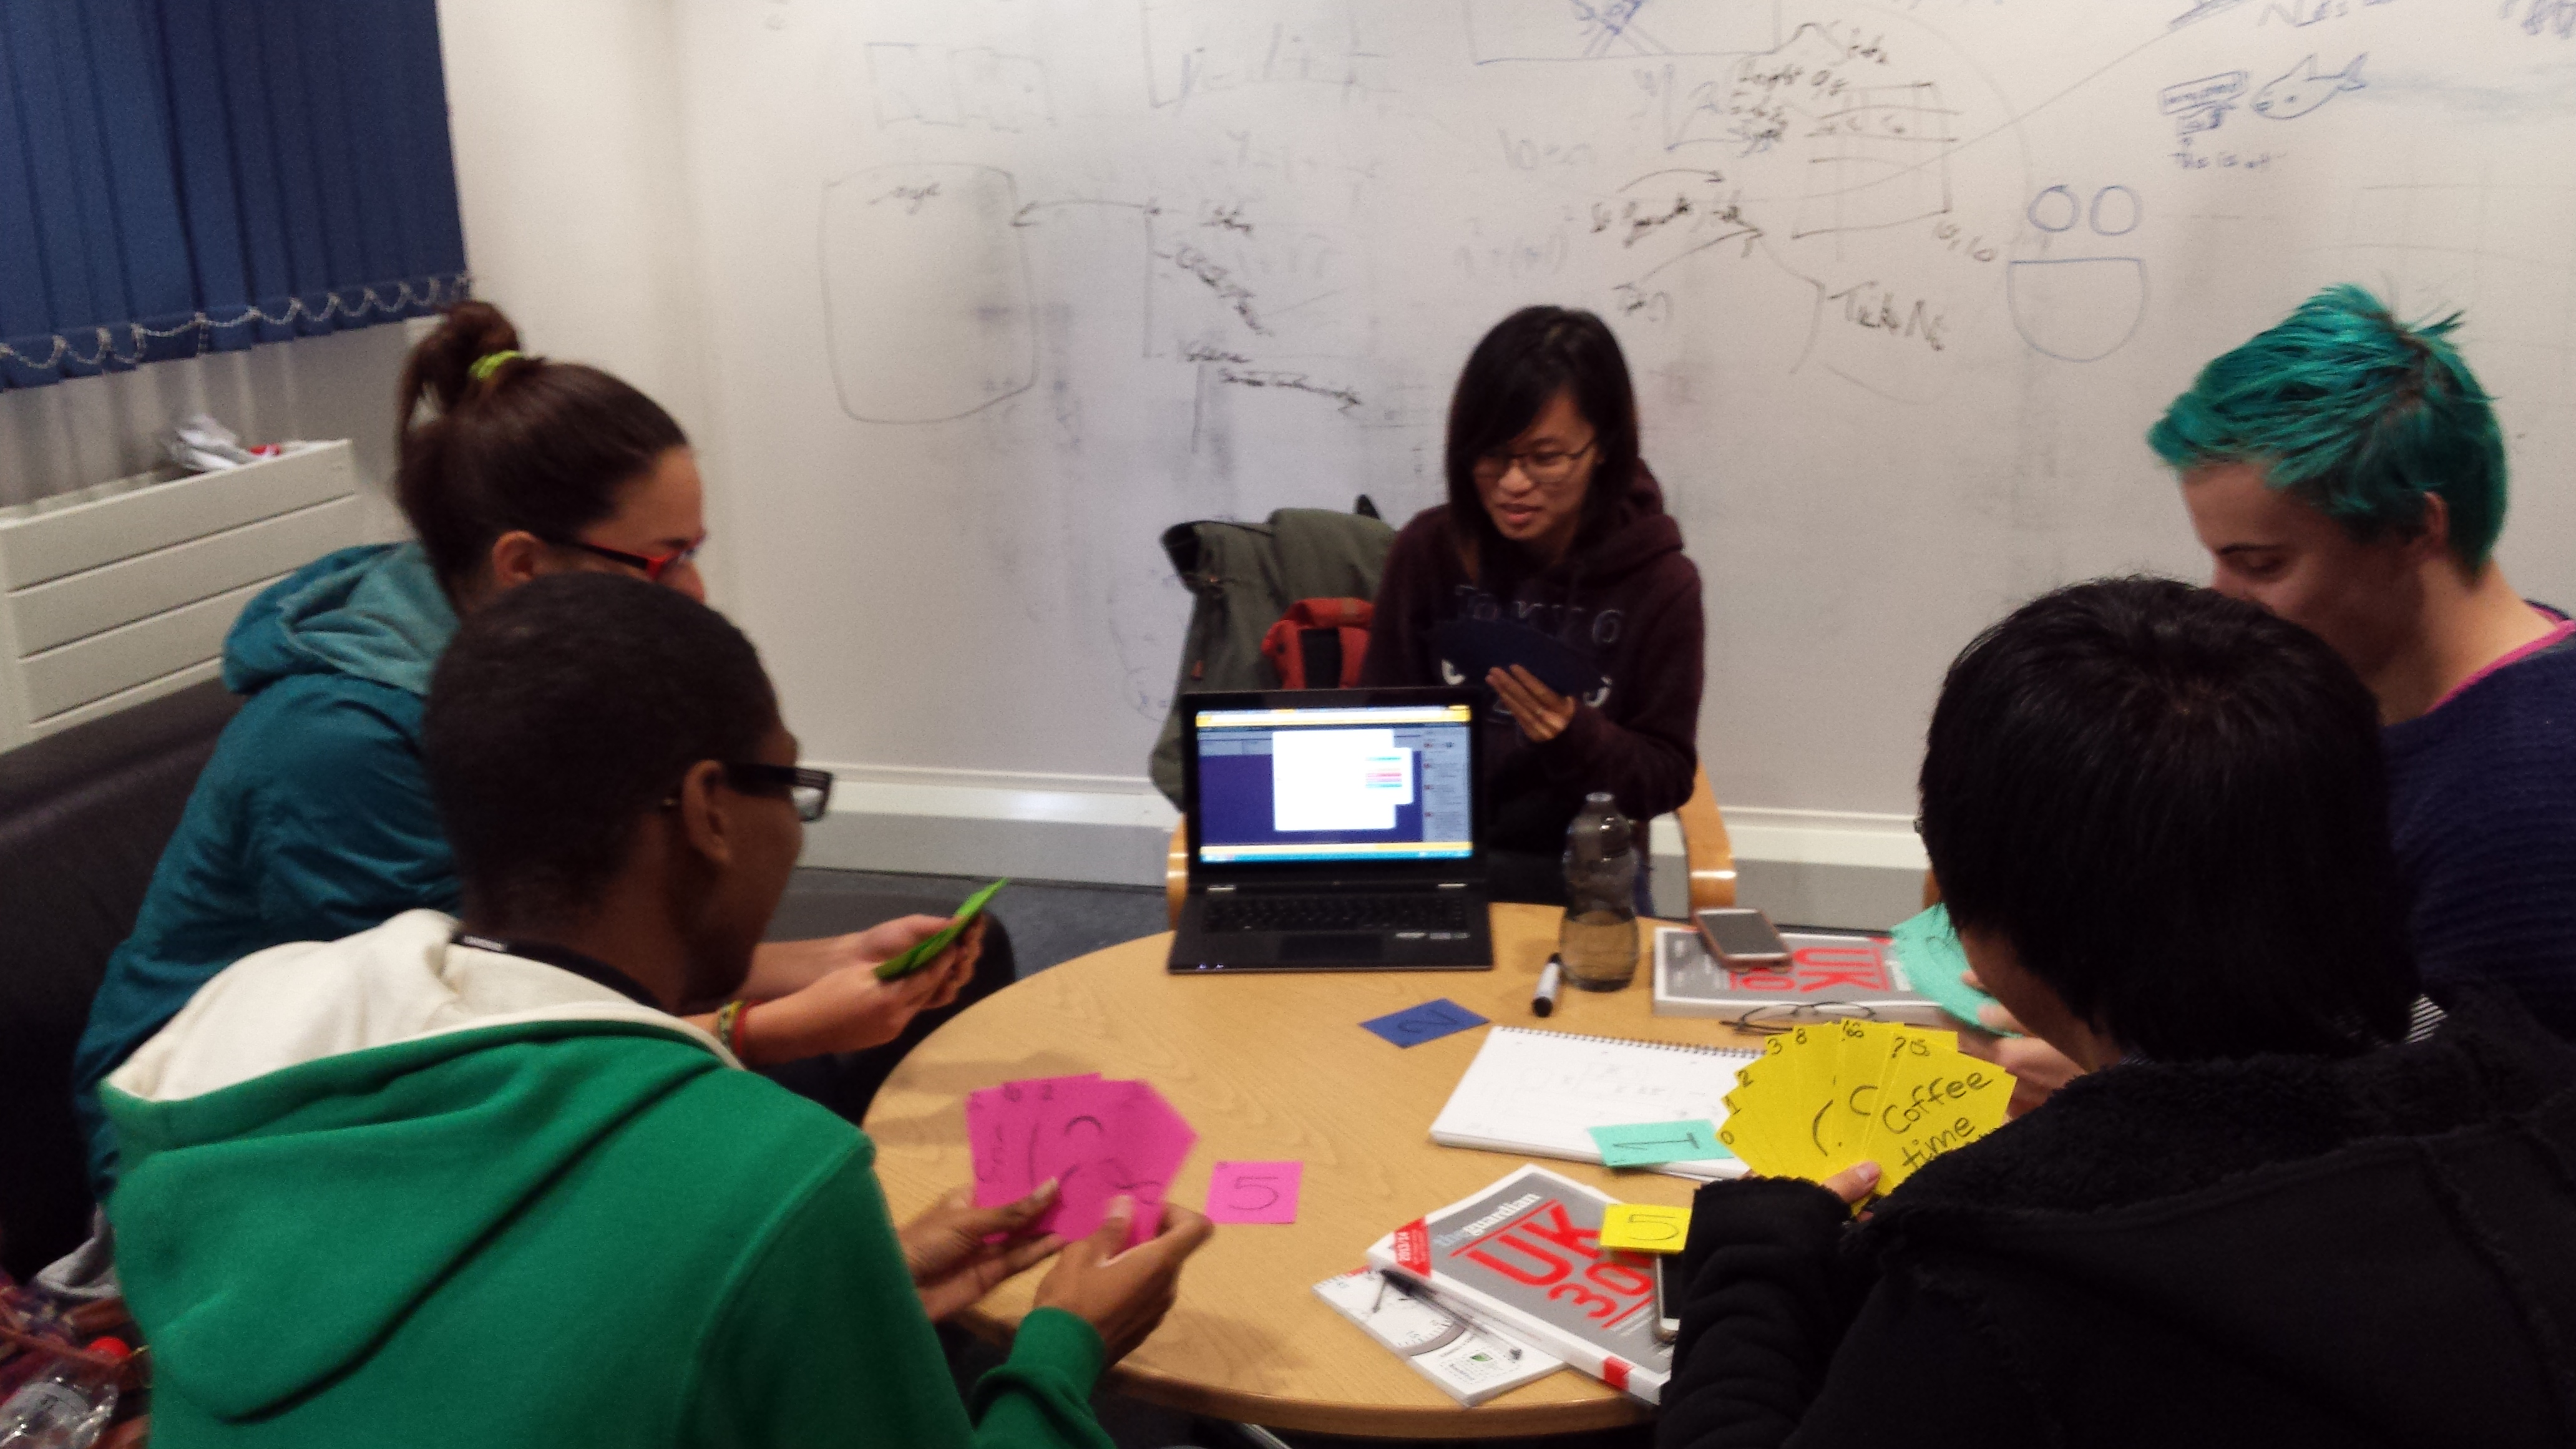
\includegraphics[height=55mm]{estimation.jpg}
\label{fig:figure1}}
\quad
\subfigure[Updated Plan]{%
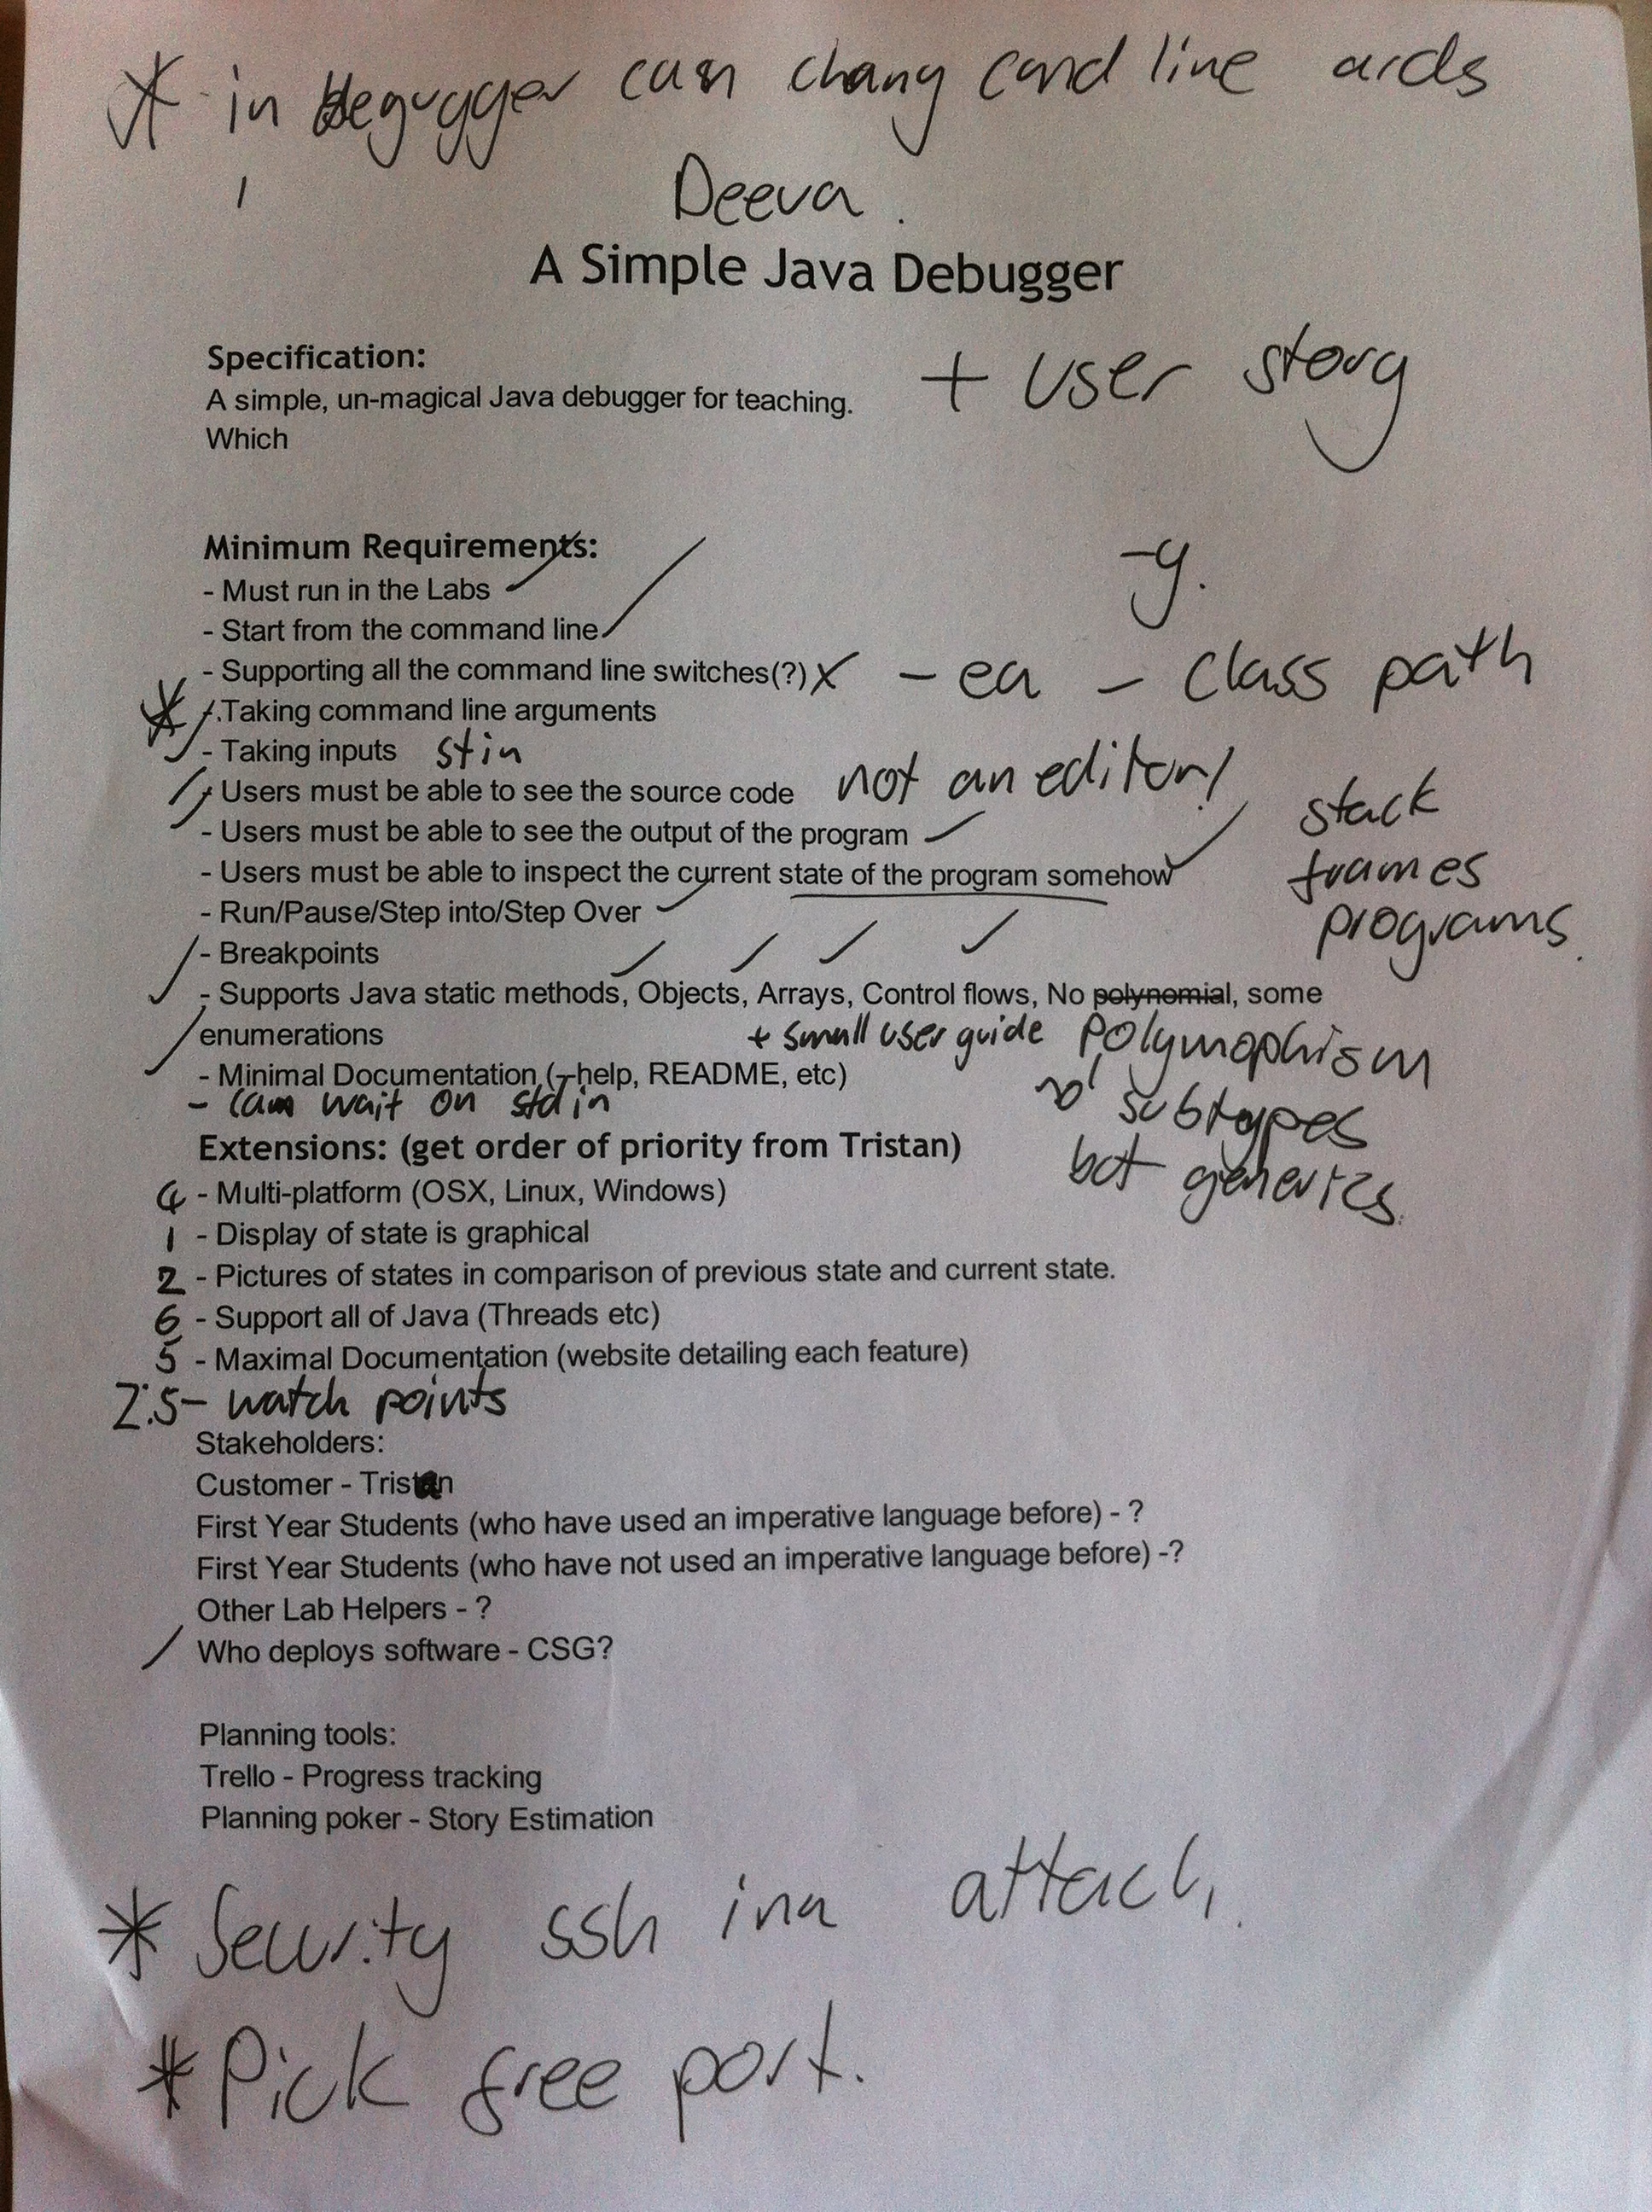
\includegraphics[height=70mm]{UpdatedPlan.jpg}
\label{fig:figure2}}
\caption{Agile Programming methods}
\label{fig:figure}
\end{figure}

\subsection{Second group meeting}
\indent In our second group meeting we discussed the research results from the previous iteration. We decided which tools would best fit our requirements and would be easy to integrate between each other. Afterwards, we created a formal plan that covers: iteration-by-iteration, all the milestones needed to deliver the product in time. For example, by week 5 we plan to have a minimal-feature demo to show Tristan and by week 7 we plan to have a basic-feature debugger that can get tested by first year students starting the `Intro to Java' course. Finally, we created new stories for each stub part of our minimal implementation. Again, we used Planning Poker to estimate the stories and then allocate them to a member of the team. For example, the card `Front end' got a score of 3 and got allocated to Krit.

We started work on an end-to-end stub solution i.e. method stubs for a basic
debugger but correct interoperability between the tools we would be using.
Later we can expand on these stub methods to function as intended.

At the same time, we were preparing a formal plan (of which the final
version is attached) for Tristan to `sign off' on. 

\subsection{Second meeting with Tristan}
After we had finished our draft plan, we met with Tristan to discuss it. We
showed him our plan and our timeline, so he could be aware of our intended
progress. He tweaked a few of the project requirements (in our plan) so it
would be more in line with his vision for the project. 

In the end we finalised on the core requirements on the project, and what
would be considered as extensions. He then prioritised the relative
importance of our extensions (i.e. which extensions to implement first when
we finish the minimal feature set). We also saw this meeting as an
opportunity to clear up any misclarifications we had with regards to the
project.

\section{Our Plan}

We elected to write a very simple plan to avoid wasting a lot of time on something that ``wouldn't survive contact with the enemy" and give us more time to iterate. 
Of course if our plan was too vague it would be useless so we had to strike a balance.
In the end our plan contained the essentials: a strong statement of the requirements (both minimum and extensions), a week by week work timetable of what we hoped to achieve, an overview of the architecture we are using and a description of the process we are using to build the software.

See the end of the report for our plan.

\section{Requirements Analysis}
Requirements analysis includes three types of activities: gathering, analyzing, and recording requirements. 

We tried to complete these steps in an iterative way\footnote{As suggested by {{\tt{http://www.agilemodeling.com/essays/agileRequirementsBestPractices.htm}}}, we avoided a ``big modeling up front'' approach instead we are using an iterative approach}. We had our first meeting with Tristan 
and we came with a preconception of features a debugger should have. He told us what makes this project different and togther we discussed the rough requirements.
After our first meeting with Tristan, we continued on improving the requirements by considering the user stories and considering first year tutorials and lab exercises as reference input to our program.
After the research step, we had a second meeting with Tristan to make a `final' decision on the core requirements and extensions. We used contract-style requirement list\footnote{\tt{http://en.wikipedia.org/wiki/Requirements\_analysis\#Contract-style\_requirement\_lists}} to document our requirements. We made sure that Tristan signed off and understood our plan.
Any change made in the plan and requirements were documented and updated using Google Drive.
As the user sees the project develop, requirements can change. Our hope is that by showing Tristan an iteration of the software every week we build the right thing.

\section{Tools}

\begin{description}
  \item[Trello] \hfill \\
As an Information Radiator\footnote{\tt{https://www.atlassian.com/wallboards/information-radiators.jsp}} we decided to use an electronic version, Trello (see Figure \ref{fig:figure4}), which allows us to track our progress and average velocity. We decided to use Trello as it fulfills most of the key features required for such a tool: it is easy to use and update, relatively flexible and allows for communications between members without too much interruption. Electronic notice boards are a manageable alternative to physical boards and we found it extremely useful when it came to keeping everyone informed on the general progress and keeping all the information in one compact environment. \\
A Trello board was created for a better project management process. There are several different swimlanes on the board: ``Proposed'', which allows all members to throw in ideas; ``In Analysis'', where people talk about their ideas and have a discussion with group members to see if the story is feasible. If it is, the card will be then moved to ``In Estimation'' where we would use planning pokers to assign the story with a complexity points. Otherwise, the story will be moved to ``Discarded''. The reason why we want to keep track of what we have discarded is that we might have thought we would not have time for it, but in reality we may have time at the end. We might want to move it back and reconsider it. After ``estimation'', the card will be assigned to group members with a set due date and be moved into ``In Development'' on the Trello board. Once the development is complete, the card should be moved into ``In Review''. This is when we need someone to review our code to improve our styling and pattern-usage.  

  \item[Planing Poker] \hfill \\
We are using Planning Poker (see Figure \ref{fig:figure3}) in order to estimate stories in each cycle of development. This method is known to avoid anchoring and will produce more accurate, less optimistic story point estimations\footnote{\tt{http://en.wikipedia.org/wiki/Planning\_poker\#Planning\_poker\_benefits}}. This technique takes some time to get used to because initially the story point bared little meaning to us. As the tasks got more concrete and we got used to compare stories against numbers in the Fibonacci sequence the poker game proved to be a very efficient method. 
For example, it helped determine when people aren't really talking about the same scope for a certain task. Frequently we have a task like ``Set up the back end." and one person gives a task a 2 while another gives it an 8. The first person thinks the task title means ``Write some stubs so the middleware can integrate." while the second thinks it means ``Implement the backend up to the minimal specification.". So using planing poker has already helped us make sure we're all on the same page. One of our group members had hand-made a set of poker cards just for estimation. It contains Fibonacci numbers up to 13 including 0 and infinity as well as ``coffee time'' if we think we need a break. 

  \item[Facebook Group] \hfill \\
  Creating a Facebook Group proved very efficient for communicating meeting times and general enquiries that were to conversational for Trello.  

  \item[Google Docs] \hfill \\
  We used it for collaborative editing on reports, plans and meeting summaries. The reason for using this was that it allows for simultaneous editing of documents.
  \item[Github and Travis CI] \hfill \\
  Github is a hosted source control which somebody else manages and is easily accessible from anywhere and also plays nicely with the hosted Continuous Integration tool - Travis CI\footnote{\tt{http://travis-ci.com/}}.


\begin{figure}[ht]
\centering
\subfigure[Trello Board]{%
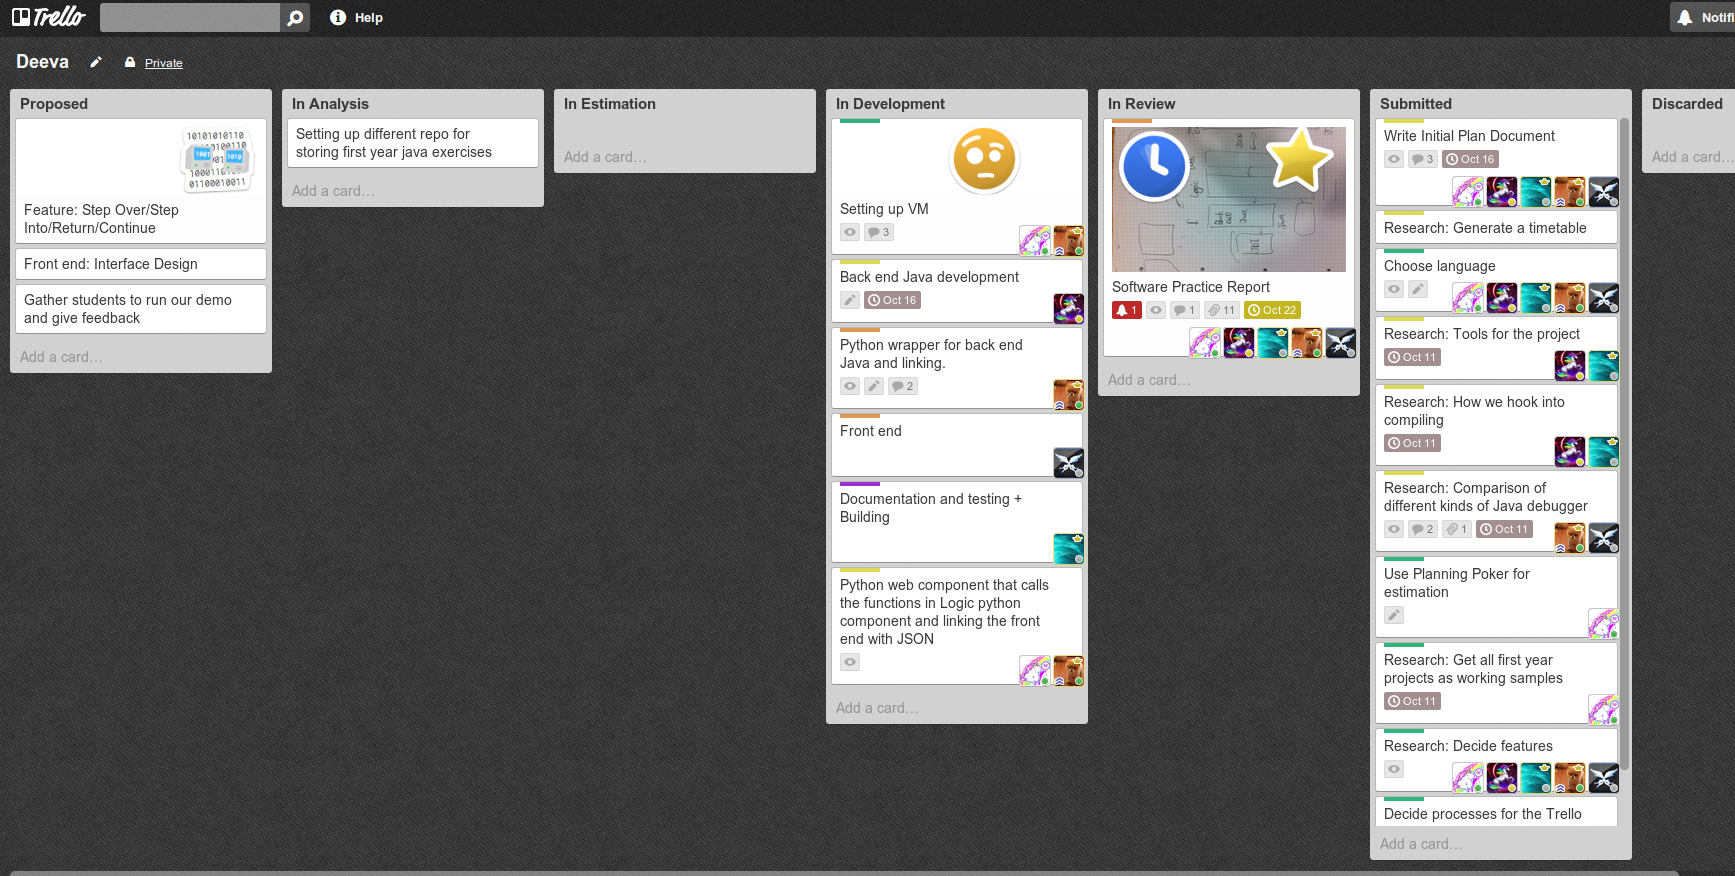
\includegraphics[height=50mm]{Trello.png}
\label{fig:figure4}}
\quad
\subfigure[Planning Poker Cards]{%
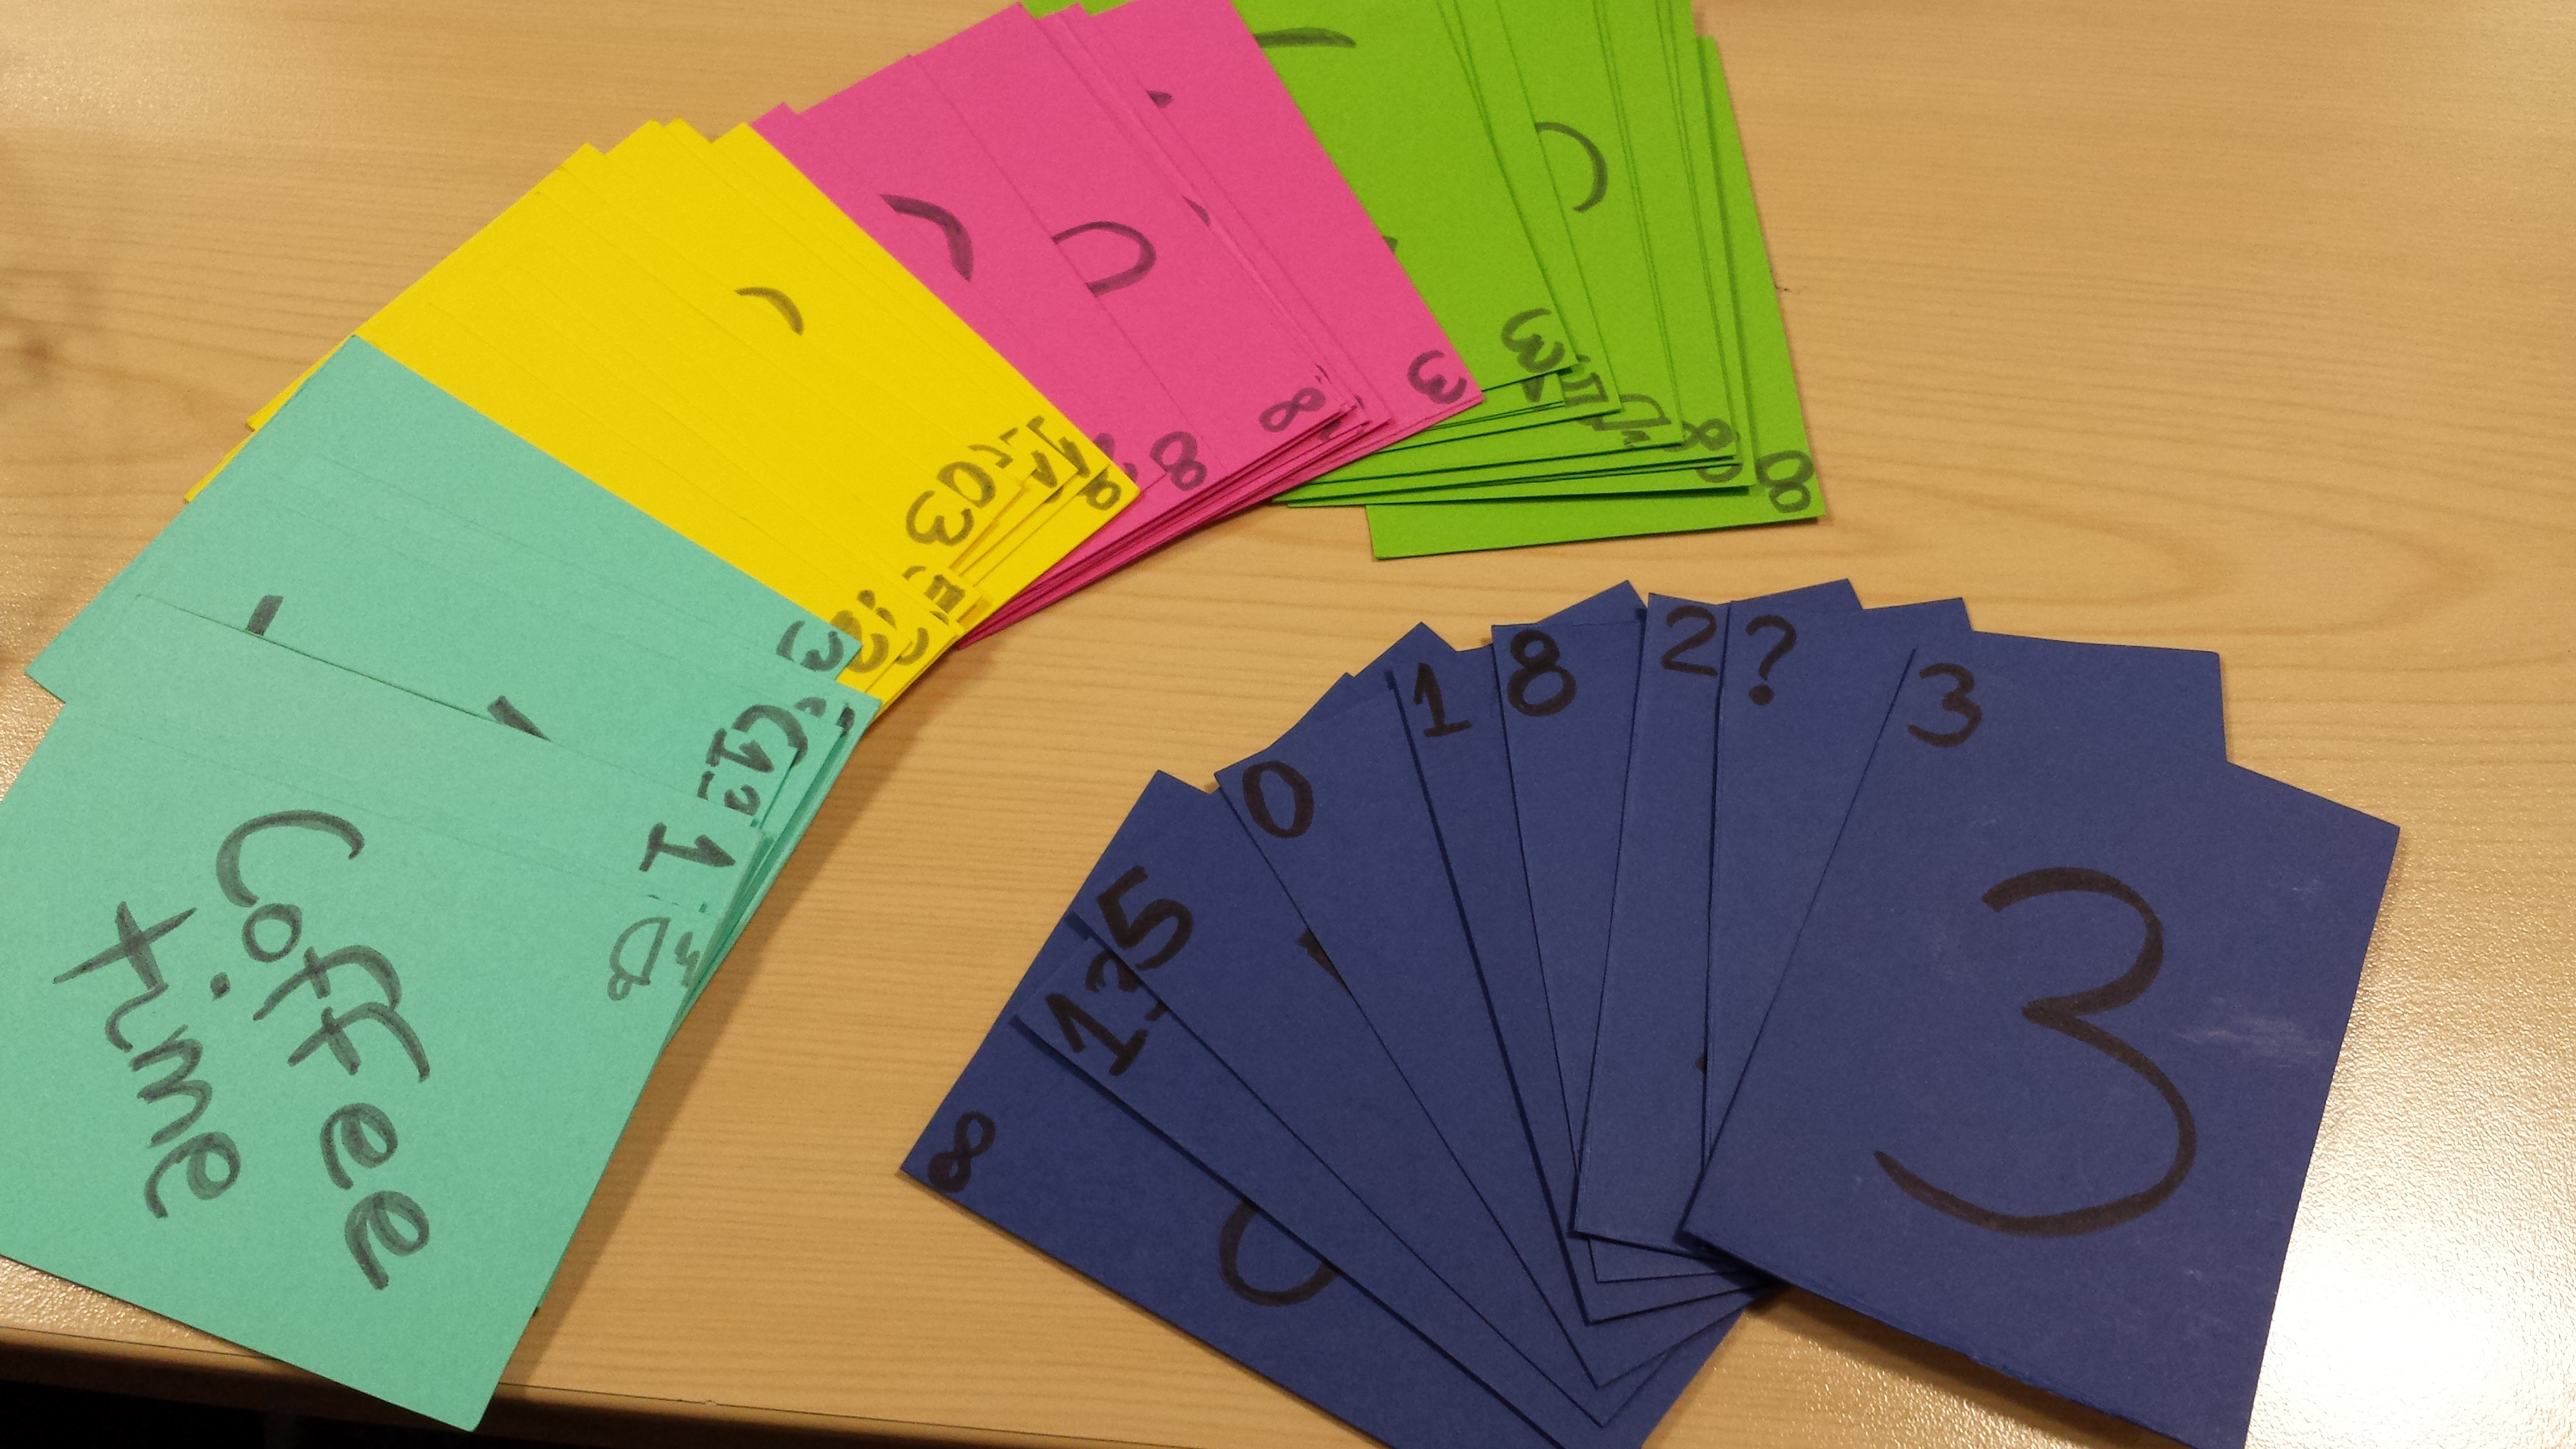
\includegraphics[height=35mm]{planningPokers.jpg}
\label{fig:figure3}}
\caption{Tools used}
\label{fig:figure}
\end{figure}

\end{description}


\end{document}
